\documentclass[12pt,a4paper]{report}
\usepackage[utf8]{inputenc}
\usepackage[russian]{babel}
\usepackage[OT1]{fontenc}
\usepackage{amsmath}
\usepackage{amsfonts}
\usepackage{amssymb}
\usepackage{graphicx}
\usepackage{listings}
\author{Панова Ксения}
\title{Лабораторная работа №2.\\
	Утилита nmap}
\begin{document}
\maketitle
\section*{Поиск активных хостов и определение открытых портов}
Задачу обнаружения хостов иногда называют пинг сканированием (ping scan). Целью всех этих запросов является получение ответов, указывающих, что IP адрес в настоящее время активен (используется хостом или сетевым устройством). В большинстве сетей лишь небольшой процент IP адресов активен в любой момент времени. Это особенно характерно для адресных пространств вида 10.0.0.0/8. Такие сети имеют 16 млн. IP адресов, но я видел, как они используются компаниями, в которых не более тысячи машин. Функция обнаружения хостов может найти эти машины в этом необъятном море IP адресов.
Если не задано никаких опций обнаружения хостов, то Nmap посылает TCP ACK пакет на порт 80 и запрос на ICMP эхо ответ кажодй целевой машине.


\begin{lstlisting}[breaklines]
root@kali:~/Documents/lab4# nmap 192.168.0.104

Starting Nmap 7.01 ( https://nmap.org ) at 2016-03-20 19:52 EDT
Nmap scan report for 192.168.0.104
Host is up (1.0s latency).
Not shown: 992 closed ports
PORT      STATE SERVICE
80/tcp    open  http
135/tcp   open  msrpc
139/tcp   open  netbios-ssn
443/tcp   open  https
445/tcp   open  microsoft-ds
554/tcp   open  rtsp
2869/tcp  open  icslap
10243/tcp open  unknown

Nmap done: 1 IP address (1 host up) scanned in 3.60 seconds
\end{lstlisting}


\begin{lstlisting}[breaklines]
root@kali:~/Documents/lab4# nmap 192.168.0.100-105

Starting Nmap 7.01 ( https://nmap.org ) at 2016-03-20 20:32 EDT

Nmap scan report for 192.168.0.100
Host is up (0.0059s latency).
All 1000 scanned ports on 192.168.0.100 are filtered

Nmap scan report for 192.168.0.101
Host is up (0.015s latency).
All 1000 scanned ports on 192.168.0.101 are filtered

Nmap scan report for 192.168.0.102
Host is up (0.0053s latency).
All 1000 scanned ports on 192.168.0.102 are filtered

Nmap scan report for 192.168.0.103
Host is up (0.081s latency).
All 1000 scanned ports on 192.168.0.103 are filtered

Nmap scan report for 192.168.0.104
Host is up (1.0s latency).
Not shown: 992 closed ports
PORT      STATE SERVICE
80/tcp    open  http
135/tcp   open  msrpc
139/tcp   open  netbios-ssn
443/tcp   open  https
445/tcp   open  microsoft-ds
554/tcp   open  rtsp
2869/tcp  open  icslap
10243/tcp open  unknown

Nmap scan report for 192.168.0.105
Host is up (0.0037s latency).
All 1000 scanned ports on 192.168.0.105 are filtered
\end{lstlisting}

Open означает, что приложение на целевой машине готово для принятия пакетов на этот порт. Filtered означает, что брандмауэр, фильтр, или что-то другое в сети блокирует порт, так что Nmap не может определить, является ли порт открытым или закрытым. Closed — не связанны в данный момент ни с каким приложением, но могут быть открыты в любой момент. Unfiltered порты отвечают на запросы Nmap, но нельзя определить, являются ли они открытыми или закрытыми. 


\begin{lstlisting}[breaklines]
root@kali:~/Documents/lab4# nmap -O 127.0.0.1

Starting Nmap 7.01 ( https://nmap.org ) at 2016-03-20 20:41 EDT
Nmap scan report for localhost (127.0.0.1)
Host is up (0.000051s latency).
Not shown: 999 closed ports
PORT     STATE SERVICE
5432/tcp open  postgresql
Device type: general purpose
Running: Linux 3.X
OS CPE: cpe:/o:linux:linux_kernel:3
OS details: Linux 3.8 - 3.19
Network Distance: 0 hops

OS detection performed. Please report any incorrect results at https://nmap.org/submit/ .
Nmap done: 1 IP address (1 host up) scanned in 2.13 seconds
\end{lstlisting}



\section*{Версии сервисов}

Для определения ОС удаленного хоста, версия которой неизвестна, необходимо иметь определенную информацию о том, как ОС известных версий реагируют на определенные виды запросов, описанных выше, иначе говоря - составить "отпечаток" стека TCP/IP операционной системы.
Алгоритм получения отпечатка стека TCP/IP следующий. Вначале проводится сканирование портов удаленного хоста с целью определения открытых портов и служб, функционирующих на исследуемом хосте. Затем проводится несколько тестов, поэтапно выполняющих опрос стека TCP/IP удаленного хоста с целью выявления   признаков, определяющих версию служб.
На основе полученных от хоста ответов составляется отпечаток, который затем сравнивается с уже имеющейся базой отпечатков, и принимается решение о типе и версии ОС исследуемого хоста.

\begin{lstlisting}[breaklines]
root@kali:~/Documents/lab4# nmap -sV 192.168.0.104

Starting Nmap 7.01 ( https://nmap.org ) at 2016-03-20 20:42 EDT
Stats: 0:00:50 elapsed; 0 hosts completed (1 up), 1 undergoing Service Scan
Service scan Timing: About 62.50% done; ETC: 20:43 (0:00:28 remaining)
Stats: 0:01:25 elapsed; 0 hosts completed (1 up), 1 undergoing Service Scan
Service scan Timing: About 62.50% done; ETC: 20:44 (0:00:49 remaining)
Nmap scan report for 192.168.0.104
Host is up (1.0s latency).
Not shown: 992 closed ports
PORT      STATE SERVICE      VERSION
80/tcp    open  http
135/tcp   open  msrpc        Microsoft Windows RPC
139/tcp   open  netbios-ssn  Microsoft Windows 98 netbios-ssn
443/tcp   open  https
445/tcp   open  microsoft-ds Microsoft Windows 7 or 10 microsoft-ds
554/tcp   open  rtsp?
2869/tcp  open  http         Microsoft HTTPAPI httpd 2.0 (SSDP/UPnP)
10243/tcp open  http         Microsoft HTTPAPI httpd 2.0 (SSDP/UPnP)
2 services unrecognized despite returning data. If you know the service/version, please submit the following fingerprints at https://nmap.org/cgi-bin/submit.cgi?new-service :
==============NEXT SERVICE FINGERPRINT (SUBMIT INDIVIDUALLY)==============
SF-Port80-TCP:V=7.01%I=7%D=3/20%Time=56EF4373%P=x86_64-pc-linux-gnu%r(GetR
SF:equest,1A,"HTTP/1\.0\x20404\x20Not\x20Found\r\n\r\n")%r(HTTPOptions,6B,
SF:"af\)\xcc\x99=\x0e\xd3\x022\x9a\xaf\x0fJ\x8e\x0e\x16\xe8\xcd\*\x84\xec\
SF:xef\xdc\x15\xbb\x02pt\xd6nU\xfar\xcfB\xa3\xd5\xe6\xe5\xa6A\xc9P\xfa\xb5
SF:g\x14\xe2k\x20\x11\x0e\xa7,\xad\xfa\xa3\xf8\t\xa6_\x84%\x12\xdb\xd0\x01
SF:>\x17\xdc\x9d\*\x13\xa8\xf9\xd6\xcf4\x15BK\x80\xf1n\x87\x8c\x8dZ\x83X\x
SF:e9\x06\?\xe4\x05r\xbb0\xe1\x9e\xf7<}\x8a\xf3\x08")%r(RTSPRequest,5C,"\x
SF:e78\xc5\x7f\xd9{i\xcd\xcf\xea5\x86W\xbf\x81W\xd6b\x0bZ\xd1\x93\xb8\x20\
SF:xdc\x7f\xa6H\xf59Vx\xea\x1e\x99\x19\$\x06\x12\x87!\x8e\x94z\xd0\xd6\x7f
SF:f\xe89\x16\x0ftU\x82\x8b\xc01\xae\xc7\xcc\xcd\x9a\xc3\x98\)F\x7f\$E\xb2
SF:\xfbp!\xde7\|\xbd\xca3H\x19v\xef\xd45\xe2k\x20\x11\x0e\xa7")%r(FourOhFo
SF:urRequest,1A,"HTTP/1\.0\x20404\x20Not\x20Found\r\n\r\n")%r(RPCCheck,60,
SF:"\xc5\xe4\xd4\x08\x19\xf2\xc1U\x0c}\xf6\xb6\rF\x0f\x7f\xb7\x98\xd1;\xf7
SF:_\x1e\xc9t\xb4h\xd1\x9f\xf9\xed{\xde\xa7F\xea\t\xa0\xe7a\xbf<\xf0\xa8\x
SF:87AU\xc4\x03\xd8i\x86\xbfd\x85\xf2;\xb0a\x1ew\xbc\xfd\ns\x88Y\xb6/\x14u
SF:\"\xab`QN\xe7l\xed:\xe38I\xe6\x9f\xc4eR\x1b\x10A~W\x1c\xddj")%r(DNSVers
SF:ionBindReq,6E,"\xd87h\x96\x9cT\?~\x9a\x0f\x91\xc4\x15\x9f\x8b\x01C\xc5\
SF:x91w\+p\xbam\xe7H\x9e\xc8\xc3\xa8\x95\xbbC\xff\xc5\x20\x86\x92\xf5\x01\
SF:xc5\xf7\x89m\xf4\xd1\x85\xbb\x96\x8f\xf4\xd5\x02\x0b@\xb1\.GLM\x1aC\x18
SF:\xa9\xc6\xff\xa4\xc52{\xf0\xa1\^\xb7\xfc=J\xb3\xc8\x99\xf6oT\xb5b\xeb\x
SF:a0\x91\x8e'\xac-z#x\x89&\xdf\x04\xa5\x92\[P\x81\xbe\x97\\\x1d\xaa\x93")
SF:%r(DNSStatusRequest,3C,"\x87\x12AZ=\xa4\xaf\xdfi\x1b\n\xa2\xaeM\x9fd@\x
SF:cc\x04\xed\xddo\xecce\*{\x11\x16n%\t\xca\+\x067>\x93I\x87mq\xce\xbe\xa9
SF:g\xf0\xf8\x10A~W\x1c\xddjS\xe89\x16\x0f")%r(SSLSessionReq,44,"\xe1E\x95
SF:\xd8\x19\xff\xc0\"\x15\xd1\xbc\xa5\(\xc2\xcd\xdc\x0b\xdf\t\xdf@\xe9\x80
SF:\x059\xd2\x7f\xbd\t8\xba\x0b\xbb\xee\xf7}'-\xa3h\x8b\xa1\x81\xd9\x9d\x8
SF:b\xe8\x9d\xbd\xca3H\x19v\xef\xd45\xe2k\x20Z\x97\xdfA\x10\x1a\xc3\x13")%
SF:r(TLSSessionReq,55,"\x9b\xc4\xcfF<g\xc4\xe7\xefU\$7p\x02\xc3\xdd\xaa\xe
SF:0i\x96\]7\x7f\xfb\\\.\x1d\xf5\x86\xa7\x18/\xa4\x9f\x98\xac\x9d:\x83\x84
SF:\xdf\xe7\xd9\x07P6\x9d\xb0l\xed:\xe38I\xe6\x9f\xc4eR\x1b\x10A~W\x1c\xdd
SF:jS\xe89\x16\x0ftU\x82\x8b\xc0\xc62\+\xdf\xe2\x9d\xa0\(");
==============NEXT SERVICE FINGERPRINT (SUBMIT INDIVIDUALLY)==============
SF-Port443-TCP:V=7.01%I=7%D=3/20%Time=56EF4378%P=x86_64-pc-linux-gnu%r(SSL
SF:SessionReq,46,"\xeeE\^\xc9\xf8k\xc7\xfa\0\xcd\xc5\x96\x85U\xc2\xc2\x88`
SF:\xb7\xed03\xc0bXTv:\r5Kuh\xdcF\xb1\(\xea\$\x1dc\x11\x1c\xf1J\xb5\x02\xa
SF:3\xf7<}\x8a\xf3\x08\xd96\xaf\x94\xf5\xa2\+\xe0r\x17J\xc7\x14YUE")%r(TLS
SF:SessionReq,57,"\x92_\x0e\x8a\x98\x9b\x04t\xb5v\x03\xbc\x83B\xeeJ\x8e\xa
SF:5\$>D\x83\xfb\xe0\xfe}\xb3>\x8b\xba\x16\xf3\x89\xde\xe0\xde\xce\xda\xdb
SF:\x14\xf3P\(\|\xe6\xabmQ\x0b@\xb1\.GLM\x1aC\x18\xa9\xc6\xff\xa4\xc52{\xf
SF:0\xa1\^\xb7\xfc=J\xb3\xc8\x99\xf6oT\xb5\x9f\xd7\xe4\\HT\x92\xb7")%r(SSL
SF:v23SessionReq,42,"K\x92\x83\xac#\x9a0\n\xb3\xd8'r\xf1\xed\xca\xdc\xd4\x
SF:c4\xe0f&\xc1\xf4\xe2\x98\x169V\xbe\x92\+\x0cN\xb5\x10@\0\x1br\x0e\xcdB\
SF:$\xe1yMy\xf6\xc8\x99\xf6oT\xb5b\xeb\xa0\x91\x8e'\xac-z#x\x89")%r(GetReq
SF:uest,1A,"HTTP/1\.0\x20404\x20Not\x20Found\r\n\r\n")%r(HTTPOptions,5C,"/
SF:\xcc\xa4B\x05\x909\xe1\^\xb7\xc9aO\xda\x12E\xb0\.\xa0\x19\x04\xad\x1d\x
SF:05\xfa\x18V\*\xf2\xca\x15\xba\xf3\xc9i\xba\x8c\xce\xc9\xe1\xd1Y\^4\x81\
SF:x13\xbc>\xa8\xf9\xd6\xcf4\x15BK\x80\xf1n\x87\x8c\x8dZ\x83X\xe9\x06\?\xe
SF:4\x05r\xbb0\xe1\x9e\xf7<}\x8a\xf3\x08\xd96\xaf\x94\xf5\xa2\+\xe0\xd1\xc
SF:eg")%r(RTSPRequest,4E,"\xd7j\x83}\x07\x15\xb2\xa3\xc0\x93P\xb8p\x7f\xb2
SF:42\x80\x11y\x8eZ\x01\xb1\xc2\xb5\^\x1a-\xedv\x02\xdf\xda\x9b\xc8\x06\xf
SF:4\xf4\xdeUN-u\x10\xe1\x814\x20\x11\x0e\xa7,\xad\xfa\xa3\xf8\t\xa6_\x84%
SF:\x12\xdb\xd0\x01>\x17\xdc\x9d\*\x13\xa8\xf9\xd6\xcf4\x15")%r(RPCCheck,3
SF:0,"\xad\xa6\xb5\x19w\xb4\xcf\xfe\xba\xf8\xcf\xd0u\xa8\xdd~\x9elRB\xdd\x
SF:1f\x16\xd9\xb5R\xe5\x02a}\xe7\x18\xdf\?~\xe0o\x9b\x10a}\xad\xf7G\xc1\xd
SF:3k\x02")%r(DNSVersionBindReq,53,"7w\xf9\xa0\x7fbQ~o\x8bC\x87o\\\xc5\xfd
SF:\x19k\xaf\xf3\xa3\xb6R5X\xf4\xf5\x92\x9e\xb3~\x8b\xa5\xbf\xec0v\]\xf2\$
SF:\x0c\)\x15Q\xdc\)C@\?\xe4\x05r\xbb0\xe1\x9e\xf7<}\x8a\xf3\x08\xd96\xaf\
SF:x94\xf5\xa2\+\xe0\xd1\xceg\xecm\xbac\xb8\xc9f\x1fD\xe5")%r(DNSStatusReq
SF:uest,30,"yL\xd0\xe1f\xe3=r\xa1\xb6\x86Kv\xc4\xf5!6p\xabc\xc4\^I\t\xca\x
SF:fc\xaa\x88\x1ez\*\xa9j\x042\x81x\xea\xa5\xd0\xd2\x1ese\xaf\xf9k\x97")%r
SF:(Kerberos,54,"\xca\xee\x85F\xc0\xdc\xa7\xa7F\xfb\xb8\xea'R2\xe9\x90\xe0
SF:\xda\xd5Q\xf2\x18N\xb0B\xe29\xc2\+\x9e0;\x18\xb8I\x8a\^\xfb\x05\xa2w\xb
SF:9@\xc0'\x1be\x1ew\xbc\xfd\ns\x88Y\xb6/\x14u\"\xab`QN\xe7l\xed:\xe38I\xe
SF:6\x9f\xc4e\x89\|\n\xbfb\x06\xbe\xb8");
Service Info: OSs: Windows, Windows 98; CPE: cpe:/o:microsoft:windows, cpe:/o:microsoft:windows_98, cpe:/o:microsoft:windows_7

Service detection performed. Please report any incorrect results at https://nmap.org/submit/ .
Nmap done: 1 IP address (1 host up) scanned in 123.06 seconds
\end{lstlisting}

Не зависимо от того, насколько технически грамотно реализована система определения версий, от нее не будет никакого толка, пока не наберется внушительная база отпечатков различных сервисов. В настоящее время существует база, которая содержит десятки тысяч отпечатков различных операционных систем и устройств. Чтобв определить, какой службе и версии соответствует отпечаток, проводятся специальные тесты.
Если служба отвечает на один или более тестов, а Nmap не может определить ее, он выведет отпечаток службы наподобие этого:
\begin{lstlisting}[breaklines]
SF:uest,30,"yL\xd0\xe1f\xe3=r\xa1\xb6\x86Kv\xc4\xf5!6p\xabc\xc4\^I\t\xca\x
SF:9@\xc0'\x1be\x1ew\xbc\xfd\ns\x88Y\xb6/\x14u\"\xab`QN\xe7l\xed:\xe38I\xe
\end{lstlisting}
Это значит, что такой службы нет в базе.




\section*{Изучение файлов nmap-services, nmap-os-db, nmap-service-probes}

\subsection*{nmap-services}
Содержит в себе все возможные порты, свыше 2200 называний общеизвестных служб, соответсвующие некоторым портам, котором
напротив каждого номера обнаруженного порта nmap укажет возможное назначение этого порта: относится ли он к почтовому серверу (SMTP), веб-серверу (HTTP) или к службе DNS
\begin{lstlisting}[breaklines]
at 4.txt 
# THIS FILE IS GENERATED AUTOMATICALLY FROM A MASTER - DO NOT EDIT.
# EDIT /nmap-private-dev/nmap-services-all IN SVN INSTEAD.
# Well known service port numbers -*- mode: fundamental; -*-
# From the Nmap Security Scanner ( http://nmap.org )
#
# $Id: nmap-services 35292 2015-10-02 07:52:30Z fyodor $
#
# Derived from IANA data and our own research
# 
# This collection of service data is (C) 1996-2011 by Insecure.Com
# LLC.  It is distributed under the Nmap Open Source license as
# provided in the COPYING file of the source distribution or at
# http://nmap.org/data/COPYING .  Note that this license
# requires you to license your own work under a compatable open source
# license.  If you wish to embed Nmap technology into proprietary
# software, we sell alternative licenses (contact sales@insecure.com).
# Dozens of software vendors already license Nmap technology such as
# host discovery, port scanning, OS detection, and version detection.
# For more details, see http://nmap.org/book/man-legal.html
#
# Fields in this file are: Service name, portnum/protocol, open-frequency, optional comments
#
tcpmux	1/tcp	0.001995	# TCP Port Service Multiplexer [rfc-1078]
tcpmux	1/udp	0.001236	# TCP Port Service Multiplexer
compressnet	2/tcp	0.000013	# Management Utility
compressnet	2/udp	0.001845	# Management Utility
compressnet	3/tcp	0.001242	# Compression Process
compressnet	3/udp	0.001532	# Compression Process
unknown	4/tcp	0.000477
rje	5/udp	0.000593	# Remote Job Entry
unknown	6/tcp	0.000502
echo	7/sctp	0.000000
echo	7/tcp	0.004855
echo	7/udp	0.024679
unknown	8/tcp	0.000013
discard	9/sctp	0.000000	# sink null
discard	9/tcp	0.003764	# sink null
discard	9/udp	0.015733	# sink null
unknown	10/tcp	0.000063
systat	11/tcp	0.000075	# Active Users
systat	11/udp	0.000577	# Active Users
unknown	12/tcp	0.000063
daytime	13/tcp	0.003927
daytime	13/udp	0.004827
unknown	14/tcp	0.000038
netstat	15/tcp	0.000038
unknown	16/tcp	0.000050
qotd	17/tcp	0.002346	# Quote of the Day
qotd	17/udp	0.009209	# Quote of the Day
msp	18/udp	0.000610	# Message Send Protocol
chargen	19/tcp	0.002559	# ttytst source Character Generator
chargen	19/udp	0.015865	# ttytst source Character Generator
ftp-data	20/sctp	0.000000	# File Transfer [Default Data]
ftp-data	20/tcp	0.001079	# File Transfer [Default Data]
ftp-data	20/udp	0.001878	# File Transfer [Default Data]
ftp	21/sctp	0.000000	# File Transfer [Control]
ftp	21/tcp	0.197667	# File Transfer [Control]
ftp	21/udp	0.004844	# File Transfer [Control]
ssh	22/sctp	0.000000	# Secure Shell Login
ssh	22/tcp	0.182286	# Secure Shell Login
ssh	22/udp	0.003905	# Secure Shell Login
telnet	23/tcp	0.221265
telnet	23/udp	0.006211
priv-mail	24/tcp	0.001154	# any private mail system
priv-mail	24/udp	0.000329	# any private mail system
smtp	25/tcp	0.131314	# Simple Mail Transfer
smtp	25/udp	0.001285	# Simple Mail Transfer
rsftp	26/tcp	0.007991	# RSFTP
nsw-fe	27/tcp	0.000138	# NSW User System FE
nsw-fe	27/udp	0.000395	# NSW User System FE
unknown	28/tcp	0.000050
msg-icp	29/tcp	0.000025	# MSG ICP
msg-icp	29/udp	0.000560	# MSG ICP
unknown	30/tcp	0.000527
\end{lstlisting}



\subsection*{nmap-service-probes}

После того как какие-либо TCP и/или UDP были обнаружены, Nmap начинает "опрашивать" эти порты, чтобы определить, какие же приложения (службы) их действительно используют. База данных nmap-service-probes содержит запросы для обращения к различным службам и соответствующие выражения для распознавания и анализа ответов. Nmap пытается определить протоколо службы (напр. FTP, SSH, Telnet, HTTP), имя приложения (e.g. ISC BIND, Apache httpd, Solaris telnetd), номер версии, имя хоста, тип устройства (напр. принтер, роутер), семейство ОС (напр. Windows, Linux) и иногда различные детали типа возможно ли соединится с X сервером, версию протокола SSH

Как принято в файлах ОС UNIX, nmap-service-probes состоит из строк. Строки, начинающиеся с символа «hash» (\#) воспринимаются как комментарии и игнорируются обработчиком. Пустые строки также не обрабатываются. Строки, подлежащие обработке, должны содержать следующие директивы:

Probe <protocol> <probename> <probesendstring>

Пример:
\begin{lstlisting}[breaklines]
Probe TCP GetRequest q|GET / HTTP/1.0\r\n\r\n|
Probe UDP DNSStatusRequest q|\0\0\x10\0\0\0\0\0\0\0\0\0|
Probe TCP NULL q||
\end{lstlisting}


Директива «probe» (тест) указывает Nmap, какие данные отправлять в процессе определения служб. Аргументы этой директивы следующие:

Protocol – тип протокола. Может быть указан один из протоколов TCP или UDP. Nmap будет использовать только те тесты, тип протокола которых совпадает с рабочтм протоколом проверяемой службы.

Probename – название теста. Используется в отпечатке службы для указания, на какой тест был получен ответ. Название может быть произвольным (удобным для пользователя).

Probestring –строка, используемая для тестового запроса. Должна начинаться и заканчиваться символом-ограничителем «q». Между ограничителями находится непосредственно сама строка, передаваемая в качестве теста. Эта строка имеет формат, аналогичный строкам языков C или Perl, и может содержать стандартные escape-последовательности: \begin{verbatim}\\ \0 \a \b \f \n \r \t \v \xHH 
\end{verbatim}. В последнем примере показано, что тестовая строка может быть пустой. Это и есть тот самый «нуль-тест», при котором данные на порт не отправляются.



match <service> <pattern> [versioninfo]

Пример:
\begin{lstlisting}[breaklines]
match domain m|^\0\0\x90\x04\0\0\0\0\0\0\0\0|
match argus m|^\x80\x01\0\x80\0\x80\0\0\xe5az\xcb
\0\0\0\0J...............\x02\0\x01\0\0<\x01
,.......\0...\0\0\0\0\x01\0\0\0\0\0\0\0\0\0
\0\0\0\0\0\0\0\0\0\0\0\0\0\0\0\0\0\0\0\0\0
\0\0\0\0\0\0\0\0\0\0\0\0\0\0\0\0\0\0\0\0\0
\0\0\0\0\0\0\0\0\0\0\0\0\0\0\0\0\0\xff\xff
\xff\xff\x01\x04\0.\0\x80\x08|s p/Argus network analyzer/ v/3.0/
match ssh m|^SSH-([\d.]+)-OpenSSH[_-]([\w.]+)\r?\n|i p/OpenSSH/ v/$2/ i/protocol $1/ cpe:/a:openbsd:openssh:$2/
\end{lstlisting}

Директива «match» указывает Nmap на то, как точно определить службу, используя полученный ответ на запрос, отправленный предыдущей директивой. Эта директива используется в случае, когда полученный ответ полностью совпадает с шаблоном. При этом тестирование порта считается законченным, а при помощи дополнительных спецификаторов Nmap строит отчет о названии приложения, номере версии и дополнительной информации, полученной в ходе проверки. Директива имеет следующие аргументы:

Service – название службы, для которой приведен шаблон. Например, ssh, smtp, http, или SNMP.

Pattern – шаблон, с которым должен совпадать полученный ответ. Формат шаблона аналогичен принятому в языке Perl, и имеет следующий синтаксис: «m/[regex]/[opts]». Литерал «m» указывает на начало строки. Прямой слэш ('/') является разделителем, вместо которого может быть подставлен любой печатаемый символ (при этом вместо второго слэша должен быть подставлен такой же символ). Regex – это регулярное выражение, принятое в языке Perl. В настоящее время поддерживаются только две опции – это 'i' (снимает чувствительность выражения к регистру) и 's', включающая символ перевода строки в спецификаторе типа '.' .

Versioninfo – это поле имеет следующий формат: 
\begin{lstlisting}[breaklines]
v/vendorproductname/version/info/\end{lstlisting}
, где слэш может быть заменен любым разделителем. Любое из трех полей может быть пустым. Кроме этого, поле само может быть пустым, и это означает, что дополнительная информация о службе отсутствует. Поле vendorproductname содержит название производителя и имя службы, например, «Sun Solaris rexecd», «ISC Bind named», или «Apache httpd». Поле version содержит «номер» версии (в кавычках потому, что может обозначаться не числовым значением, а напротив, состоять из нескольких слов). Поле info содержит дополнительную полезную информацию, которая может пригодиться на этапе сканирования (например, номер протокола сервера ssh).


softmatch <service> <pattern>

Примеры:
\begin{verbatim}
softmatch ssh m|^SSH-([\d.]+)-| i/protocol $1/
softmatch ppp m|^\x7e\xff\x7d\x23.*\x7e|
\end{verbatim}
Директива softmatch имеет формат, аналогичный директиве match. Основное отличие заключается в том, что после совпадения принятого ответа с одним из шаблонов softmatch, тестирование будет продолжено с использованием только тех тестов, которые относятся к определенной шаблоном службе. Тестирование порта будет идти до тех пор, пока не будет найдено строгое соответствие («match») или не закончатся все тесты для данной службы. Аргументы те же самые, только отсутствует versioninfo.

ports <portlist> и sslports <portlist>

Пример:
\begin{lstlisting}[breaklines]
ports 21,23,35,43,79,98,110,113,119,199,214,264,449,
505,510,540,587,616,628,666,731,771,782,1000,1010,
1040-1043,1080,1212,1220,1248,1302,1400,1432,1467,
1501,1505,1666,1687-1688,2010,2024,2600,3000,3005,
3128,3310,3333,3940,4155,5000,5400,5432,5555,5570,
6112,6667-6670,7144,7145,7200,7780,8000,8138,9000-9003,
9801,11371,11965,13720,15000-15002,18086,19150,
26214,26470,31416,30444,34012,56667
sslports 989,990,992,995
\end{lstlisting}
Эта директива группирует порты, которые обычно закрепляются за идентифицируемой данным тестом службой. Синтаксис представляет собой упрощенный формат опции ‘-p’. Директива sslports указывает порты, обычно используемые совместно с SSL

totalwaitms <milliseconds>

Пример:
\begin{verbatim}
totalwaitms 5000
\end{verbatim}
Редко используемая директива. Она указывает, сколько времени (в миллисекундах) необходимо ждать ответ, прежде чем прекратить тест службы.



\subsection*{nmap-os-db}

Одна из наиболее известных функциональных возможностей Nmap это удаленное определение ОС на основе анализа работы стека TCP/IP. Nmap посылает серию TCP и UDP пакетов на удаленный хост и изучает практически каждый бит в ответах. После проведения дюжины тестов, таких как TCP ISN выборки, поддержки опций TCP, IP ID выборки, и анализа продолжительности процедуры инициализации, Nmap сравнивает результаты со своей nmap-os-db базой данных, состоящей из более чем тысячи известных наборов типичных результатов для различных ОС и, при нахождении соответствий, выводит информацию об ОС. Каждый набор содержит свободное текстовое описание ОС и классификацию, в которой указаны название производителя (напр. Sun), название ОС (напр. Solaris), поколение ОС (напр. 10), и тип устройства (). OS, and a classification which provides the vendor name (e.g. Sun), underlying OS (e.g. Solaris), OS generation (e.g. 10), and device type (для общих целей, роутер, коммутатор (switch), игровая консоль и т.д.).

Пример:
\begin{lstlisting}[breaklines]
# Windows 10 build 10240
Fingerprint Microsoft Windows 10 build 10240
Class Microsoft | Windows | 10 | general purpose
CPE cpe:/o:microsoft:windows_10 auto
SEQ(SP=104-10E%GCD=1-6%ISR=106-110%TI=I%CI=I%II=I%SS=S%TS=A)
OPS(O1=M5BCNW8ST11%O2=M5BCNW8ST11%O3=M5BCNW8NNT11%O4=M5BCNW8ST11%O5=M5BCNW8ST11%O6=M5BCST11)
WIN(W1=2000%W2=2000%W3=2000%W4=2000%W5=2000%W6=2000)
ECN(R=Y%DF=Y%T=7B-85%TG=80%W=2000%O=M5BCNW8NNS%CC=N%Q=)
T1(R=Y%DF=Y%T=7B-85%TG=80%S=O%A=S+%F=AS%RD=0%Q=)
T2(R=Y%DF=Y%T=7B-85%TG=80%W=0%S=Z%A=S%F=AR%O=%RD=0%Q=)
T3(R=Y%DF=Y%T=7B-85%TG=80%W=0%S=Z%A=O%F=AR%O=%RD=0%Q=)
T4(R=Y%DF=Y%T=7B-85%TG=80%W=0%S=A%A=O%F=R%O=%RD=0%Q=)
T5(R=Y%DF=Y%T=7B-85%TG=80%W=0%S=Z%A=S+%F=AR%O=%RD=0%Q=)
T6(R=Y%DF=Y%T=7B-85%TG=80%W=0%S=A%A=O%F=R%O=%RD=0%Q=)
T7(R=Y%DF=Y%T=7B-85%TG=80%W=0%S=Z%A=S+%F=AR%O=%RD=0%Q=)
U1(DF=N%T=7B-85%TG=80%IPL=164%UN=0%RIPL=G%RID=G%RIPCK=G%RUCK=G%RUD=G)
IE(DFI=N%T=7B-85%TG=80%CD=Z)
\end{lstlisting}


\section*{Добавление новой сигнатуры службы в файл nmap-service-probes}

Для добавления новой сигнатуры создадим минимальный tcp server и добитьемся, чтобы при сканировании nmap указывал для него название и версию.

Исходный код tcp-сервера

\begin{lstlisting}[breaklines]
#include <sys/types.h>
#include <sys/socket.h>
#include <netdb.h>
#include <stdio.h>
#include <string.h>
#include <unistd.h>
 
int main(){
    char str[100];
	char *resp = "Hello, Server 1.0\n";
    int listen_fd, comm_fd;
 
    struct sockaddr_in servaddr;
 
    listen_fd = socket(AF_INET, SOCK_STREAM, 0);
 
    bzero( &servaddr, sizeof(servaddr));
 
    servaddr.sin_family = AF_INET;
    servaddr.sin_addr.s_addr = htons(INADDR_ANY);
    servaddr.sin_port = htons(11089);
 
    bind(listen_fd, (struct sockaddr *) &servaddr, sizeof(servaddr)); 
    listen(listen_fd, 10); 

    comm_fd = accept(listen_fd, (struct sockaddr*) NULL, NULL); 
    while(1){ 
        bzero( str, 100); 
        read(comm_fd,str,100); 
        printf("Echoing back - %s",str); 
        write(comm_fd, resp, strlen(resp)+1); 
    }
}
\end{lstlisting}

\begin{lstlisting}[breaklines]
root@kali:~/Documents/lab4# nmap -sV 127.0.0.1

Starting Nmap 7.01 ( https://nmap.org ) at 2016-04-03 17:15 EDT
Nmap scan report for localhost (127.0.0.1)
Host is up (0.0000020s latency).
Not shown: 998 closed ports
PORT      STATE SERVICE     VERSION
5432/tcp  open  postgresql  PostgreSQL DB
11089/tcp open  HelloServer HelloServer 1.0
\end{lstlisting}

\section*{Сохранение вывода утилиты в формате xml}

\begin{lstlisting}[breaklines]
root@kali:~/Documents/lab4# nmap -oX out.xml -sV 127.0.0.1

Starting Nmap 7.01 ( https://nmap.org ) at 2016-04-03 17:35 EDT
Nmap scan report for localhost (127.0.0.1)
Host is up (0.0000020s latency).
Not shown: 998 closed ports
PORT      STATE SERVICE     VERSION
5432/tcp  open  postgresql  PostgreSQL DB
11089/tcp open  HelloServer HelloServer 1.0
\end{lstlisting}

\begin{lstlisting}[breaklines]
<?xml version="1.0" encoding="UTF-8"?>
<!DOCTYPE nmaprun>
<?xml-stylesheet href="file:///usr/bin/../share/nmap/nmap.xsl" type="text/xsl"?>
<!-- Nmap 7.01 scan initiated Sun Apr  3 17:35:01 2016 as: nmap -oX out.xml -sV 127.0.0.1 -->
<nmaprun scanner="nmap" args="nmap -oX out.xml -sV 127.0.0.1" start="1459719301" startstr="Sun Apr  3 17:35:01 2016" version="7.01" xmloutputversion="1.04">
<scaninfo type="syn" protocol="tcp" numservices="1000" services="
1,3-4,6-7,9,13,17,19-26,30,32-33,37,42-43,49,53,70
,79-85,88-90,99-100,106,109-111,113,119,125,135,
139,143-144,146,161,163,179,199,211-212,222,254-256,
259,264,280,301,306,311,340,366,389,406-407,416-417,
425,427,443-445,458,464-465,481,497,500,512-515,524,
541,543-545,548,554-555,563,587,593,616-617,625,631,
636,646,648,666-668,683,687,691,700,705,711,714,720,
722,726,749,765,777,783,787,800-801,808,843,873,880,
888,898,900-903,911-912,981,987,990,992-993,995,
999-1002,1007,1009-1011,1021-1100,1102,1104-1108,
1110-1114,1117,1119,1121-1124,1126,1130-1132,
1137-1138,1141,1145,1147-1149,1151-1152,1154,
1163-1166,1169,1174-1175,1183,1185-1187,1192,
1198-1199,1201,1213,1216-1218,1233-1234,1236,
1244,1247-1248,1259,1271-1272,1277,1287,1296,
1300-1301,1309-1311,1322,1328,1334,1352,1417,
1433-1434,1443,1455,1461,1494,1500-1501,1503,
1521,1524,1533,1556,1580,1583,1594,1600,1641,
1658,1666,1687-1688,1700,1717-1721,1723,1755
,1761,1782-1783,1801,1805,1812,1839-1840,
1862-1864,1875,1900,1914,1935,1947,1971-1972,
1974,1984,1998-2010,2013,2020-2022,2030
,2033-2035,2038,2040-2043,2045-2049,2065,2068,
2099-2100,2103,2105-2107,2111,2119,2121,2126,
2135,2144,2160-2161,2170,2179,2190-2191,2196,
2200,2222,2251,2260,2288,2301,2323,2366,
2381-2383,2393-2394,2399,2401,2492,2500,2522,
2525,2557,2601-2602,2604-2605,2607-2608,2638,
2701-2702,2710,2717-2718,2725,2800,2809,2811,
2869,2875,2909-2910,2920,2967-2968,2998,
3000-3001,3003,3005-3007,3011,3017,3030-3031,
3052,3071,3077,3128,3168,3211,3221,3260-3261,
3268-3269,3283,3300-3301,3306,3322-3325,3333,
3351,3367,3369-3372,3389-3390,3404,3476,3493,
3517,3527,3546,3551,3580,3659,3689-3690,3703,
3737,3766,3784,3800-3801,3809,3814,3826-3828,
3851,3869,3871,3878,3880,3889,3905,3914,3918,
3920,3945,3971,3986,3995,3998,4000-4006,4045,
4111,4125-4126,4129,4224,4242,4279,4321,4343,
4443-4446,4449,4550,4567,4662,4848,4899-4900,
4998,5000-5004,5009,5030,5033,5050-5051,5054,
5060-5061,5080,5087,5100-5102,5120,5190,5200,
5214,5221-5222,5225-5226,5269,5280,5298,5357,
5405,5414,5431-5432,5440,5500,5510,5544,5550,
5555,5560,5566,5631,5633,5666,5678-5679,5718,
5730,5800-5802,5810-5811,5815,5822,5825,5850,
5859,5862,5877,5900-5904,5906-5907,5910-5911,
5915,5922,5925,5950,5952,5959-5963,5987-5989,
5998-6007,6009,6025,6059,6100-6101,6106,6112,
6123,6129,6156,6346,6389,6502,6510,6543,6547,
6565-6567,6580,6646,6666-6669,6689,6692,6699,
6779,6788-6789,6792,6839,6881,6901,6969,
7000-7002,7004,7007,7019,7025,7070,7100,7103,
7106,7200-7201,7402,7435,7443,7496,7512,7625,
7627,7676,7741,7777-7778,7800,7911,7920-7921,
7937-7938,7999-8002,8007-8011,8021-8022,8031,
8042,8045,8080-8090,8093,8099-8100,8180-8181,
8192-8194,8200,8222,8254,8290-8292,8300,8333,
8383,8400,8402,8443,8500,8600,8649,8651-8652,
8654,8701,8800,8873,8888,8899,8994,9000-9003,
9009-9011,9040,9050,9071,9080-9081,9090-9091,
9099-9103,9110-9111,9200,9207,9220,9290,9415,
9418,9485,9500,9502-9503,9535,9575,9593-9595,
9618,9666,9876-9878,9898,9900,9917,9929,
9943-9944,9968,9998-10004,10009-10010,10012,
10024-10025,10082,10180,10215,10243,10566,
10616-10617,10621,10626,10628-10629,10778,
11089,11110-11111,11967,12000,12174,12265,
12345,13456,13722,13782-13783,14000,14238,
14441-14442,15000,15002-15004,15660,15742,
16000-16001,16012,16016,16018,16080,16113,
16992-16993,17877,17988,18040,18101,18988,
19101,19283,19315,19350,19780,19801,19842,
20000,20005,20031,20221-20222,20828,21571,
22939,23502,24444,24800,25734-25735,26214,
27000,27352-27353,27355-27356,27715,28201,
30000,30718,30951,31038,31337,32768-32785,
33354,33899,34571-34573,35500,38292,40193,
40911,41511,42510,44176,44442-44443,44501,
45100,48080,49152-49161,49163,49165,49167,
49175-49176,49400,49999-50003,50006,50300,
50389,50500,50636,50800,51103,51493,52673,
52822,52848,52869,54045,54328,55055-55056,
55555,55600,56737-56738,57294,57797,58080,
60020,60443,61532,61900,62078,63331,64623,
64680,65000,65129,65389"/>
<verbose level="0"/>
<debugging level="0"/>
<host starttime="1459719301" endtime="1459719307"><status state="up" reason="localhost-response" reason_ttl="0"/>
<address addr="127.0.0.1" addrtype="ipv4"/>
<hostnames>
<hostname name="localhost" type="PTR"/>
</hostnames>
<ports><extraports state="closed" count="998">
<extrareasons reason="resets" count="998"/>
</extraports>
<port protocol="tcp" portid="5432"><state state="open" reason="syn-ack" reason_ttl="64"/><service name="postgresql" product="PostgreSQL DB" servicefp="SF-Port5432-TCP:V=7.01%I=7%D=4/3%Time=57018C8B%P=x86_64-pc-linux-gnu%r(SMBProgNeg,85,&quot;E\0\0\0\x84SFATAL\0C0A000\0Munsupported\x20frontend\x20protocol\x2065363\.19778:\x20server\x20supports\x201\.0\x20to\x203\.0\0Fpostmaster\.c\0L1991\0RProcessStartupPacket\0\0&quot;);" method="probed" conf="10"><cpe>cpe:/a:postgresql:postgresql</cpe></service></port>
<port protocol="tcp" portid="11089"><state state="open" reason="syn-ack" reason_ttl="64"/><service name="HelloServer" product="HelloServer" version="1.0" method="probed" conf="10"/></port>
</ports>
<times srtt="2" rttvar="0" to="100000"/>
</host>
<runstats><finished time="1459719307" timestr="Sun Apr  3 17:35:07 2016" elapsed="6.79" summary="Nmap done at Sun Apr  3 17:35:07 2016; 1 IP address (1 host up) scanned in 6.79 seconds" exit="success"/><hosts up="1" down="0" total="1"/>
</runstats>
</nmaprun>
\end{lstlisting}

\section*{Исследование различных этапов работы nmap с использованием утилиты Wireshark}


На рисунке ниже представлен результат анализа сканирования порта 445.
Сначала на хост с IP-адресом 192.169.0.104 отправляется эхо-запрос для того, чтобы удостовериться в доступности хоста. После того, как мы получили ответ, отправляется запрос с пробой, соответствующей 445 порту из файла nmap-service-probes:
\begin{figure}[ht!]
\centering
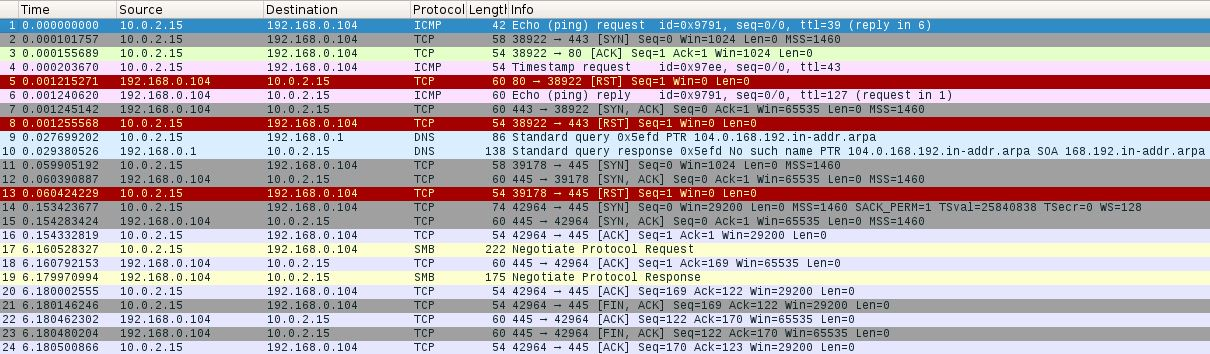
\includegraphics[width=160mm]{res/wireshark.jpg}
\caption{Сканирование порта 445\label{overflow}}
\end{figure}

\begin{lstlisting}[breaklines]
# SMB Negotiate Protocol
##############################NEXT PROBE##############################
Probe TCP SMBProgNeg q|\0\0\0\xa4\xff\x53\x4d\x42\x72\0\0\0\0\x08\x01\x40\0\0\0\0\0\0\0\0\0\0\0\0\0\0\x40\x06\0\0\x01\0\0\x81\0\x02PC NETWORK PROGRAM 1.0\0\x02MICROSOFT NETWORKS 1.03\0\x02MICROSOFT NETWORKS 3.0\0\x02LANMAN1.0\0\x02LM1.2X002\0\x02Samba\0\x02NT LANMAN 1.0\0\x02NT LM 0.12\0|
rarity 4
ports 42,88,135,139,445,660,1025,1027,1031,1112,
3006,3900,5000,5009,5432,5555,5600,7461,9102,9103,18182,27000-27010
\end{lstlisting}


В ответ целевой хост посылает сообщение, соответствующее шаблону: 

\begin{lstlisting}[breaklines]
match microsoft-ds m|^\0\0\0.\xffSMBr\0\0\0\0\x88\x01@\0\0\0\0\0\0\0\0\0\0\0\0\0\0@\x06\0\0\x01\0\x11\x07\0.\n\0\x01\0\x04\x11\0\0\0\0\x01\0\0\0\0\0\xfc\xe3\x01\0|s p/Microsoft Windows 7 or 10 microsoft-ds/ o/Windows/ cpe:/o:microsoft:windows_7/a
\end{lstlisting}
Результат:
\begin{lstlisting}[breaklines]
root@kali:~/Documents/lab4# nmap -sV -p445 192.168.0.104

Starting Nmap 7.01 ( https://nmap.org ) at 2016-04-03 21:12 EDT
Nmap scan report for 192.168.0.104
Host is up (0.00100s latency).
PORT    STATE SERVICE      VERSION
445/tcp open  microsoft-ds Microsoft Windows 7 or 10 microsoft-ds
Service Info: OS: Windows; CPE: cpe:/o:microsoft:windows_7

Service detection performed. Please report any incorrect results at https://nmap.org/submit/ .
Nmap done: 1 IP address (1 host up) scanned in 6.86 seconds
\end{lstlisting}

В случае, если пытаемся просканировать закрытый порт, когда устанавливается TCP-соединение, в ответ на пакет с установленным флагом SYN приходит пакет с флагами [RST, ACK], что является сигнаом того, что порт закрыт. Тогда nmap ищет информацию о заданном порте в nmap-services. Если в файле содержится какая-то информация о возможном сервисе на этом порте, то выводится имя этого сервиса, иначе unknown:
\begin{lstlisting}[breaklines]
msf > db_nmap 192.168.0.105 -p 41523
[*] Nmap: Starting Nmap 7.01 ( https://nmap.org ) at 2016-05-15 05:39 EDT
[*] Nmap: Nmap scan report for 192.168.0.105
[*] Nmap: Host is up (0.00046s latency).
[*] Nmap: PORT      STATE  SERVICE
[*] Nmap: 41523/tcp closed unknown
[*] Nmap: MAC Address: 08:00:27:5F:82:80 (Oracle VirtualBox virtual NIC)
[*] Nmap: Nmap done: 1 IP address (1 host up) scanned in 0.20 seconds
\end{lstlisting}
\begin{lstlisting}[breaklines]
msf > db_nmap 192.168.0.105 -p 446
[*] Nmap: Starting Nmap 7.01 ( https://nmap.org ) at 2016-05-15 05:48 EDT
[*] Nmap: Nmap scan report for 192.168.0.105
[*] Nmap: Host is up (0.00036s latency).
[*] Nmap: PORT    STATE  SERVICE
[*] Nmap: 446/tcp closed ddm-rdb
[*] Nmap: MAC Address: 08:00:27:5F:82:80 (Oracle VirtualBox virtual NIC)
[*] Nmap: Nmap done: 1 IP address (1 host up) scanned in 0.15 seconds
\end{lstlisting}

\begin{figure}[ht!]
\centering
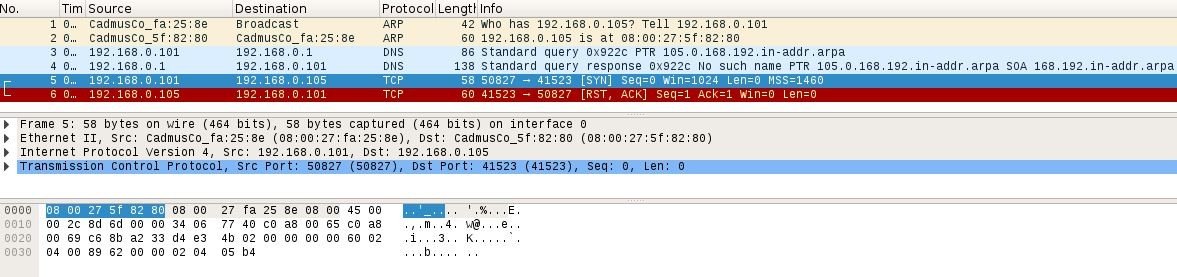
\includegraphics[width=160mm]{res/wireshark2.jpg}
\caption{Сканирование закрытого порта 41523\label{overflow}}
\end{figure}


\section*{Сканирование виртуальной машину Metasploitable2, используя db\_nmap}

Проверим содержимое базы данных эксплойтов:

\begin{lstlisting}[breaklines]
msf > search

Matching Modules
================

   Name                                                                     Disclosure Date  Rank       Description
   ----                                                                     ---------------  ----       -----------
   auxiliary/admin/2wire/xslt_password_reset                                2007-08-15       normal     2Wire Cross-Site Request Forgery Password Reset Vulnerability
   auxiliary/admin/android/google_play_store_uxss_xframe_rce                                 normal     Android Browser RCE Through Google Play Store XFO
   auxiliary/admin/appletv/appletv_display_image                                             normal     Apple TV Image Remote Control
   auxiliary/admin/appletv/appletv_display_video                                             normal     Apple TV Video Remote Control
   auxiliary/admin/atg/atg_client                                                            normal     Veeder-Root Automatic Tank Gauge (ATG) Administrative Client
...
   post/windows/recon/outbound_ports                                                         normal     Windows Outbound-Filtering Rules
   post/windows/recon/resolve_ip                                                             normal     Windows Recon Resolve IP
   post/windows/wlan/wlan_bss_list                                                           normal     Windows Gather Wireless BSS Info
   post/windows/wlan/wlan_current_connection                                                 normal     Windows Gather Wireless Current Connection Info
   post/windows/wlan/wlan_disconnect                                                         normal     Windows Disconnect Wireless Connection
   post/windows/wlan/wlan_profile                                                            normal     Windows Gather Wireless Profile
\end{lstlisting}

Сканируем Meatsploitable2:
\begin{lstlisting}[breaklines]
msf > db_nmap 192.168.0.105
[*] Nmap: Starting Nmap 7.01 ( https://nmap.org ) at 2016-05-14 22:11 EDT
[*] Nmap: Nmap scan report for 192.168.0.105
[*] Nmap: Host is up (0.000090s latency).
[*] Nmap: Not shown: 977 closed ports
[*] Nmap: PORT     STATE SERVICE
[*] Nmap: 21/tcp   open  ftp
[*] Nmap: 22/tcp   open  ssh
[*] Nmap: 23/tcp   open  telnet
[*] Nmap: 25/tcp   open  smtp
[*] Nmap: 53/tcp   open  domain
[*] Nmap: 80/tcp   open  http
[*] Nmap: 111/tcp  open  rpcbind
[*] Nmap: 139/tcp  open  netbios-ssn
[*] Nmap: 445/tcp  open  microsoft-ds
[*] Nmap: 512/tcp  open  exec
[*] Nmap: 513/tcp  open  login
[*] Nmap: 514/tcp  open  shell
[*] Nmap: 1099/tcp open  rmiregistry
[*] Nmap: 1524/tcp open  ingreslock
[*] Nmap: 2049/tcp open  nfs
[*] Nmap: 2121/tcp open  ccproxy-ftp
[*] Nmap: 3306/tcp open  mysql
[*] Nmap: 5432/tcp open  postgresql
[*] Nmap: 5900/tcp open  vnc
[*] Nmap: 6000/tcp open  X11
[*] Nmap: 6667/tcp open  irc
[*] Nmap: 8009/tcp open  ajp13
[*] Nmap: 8180/tcp open  unknown
[*] Nmap: MAC Address: 08:00:27:5F:82:80 (Oracle VirtualBox virtual NIC)
[*] Nmap: Nmap done: 1 IP address (1 host up) scanned in 0.24 seconds
\end{lstlisting}

\section*{Описание работы записей из файла nmap-service-probes и скрипта из состава Nmap}

* Распознавание сервиса ssl
\begin{lstlisting}[breaklines]
Probe TCP SSLSessionReq q|\x16\x03\0\0S\x01\0\0O\x03\0?G\xd7\xf7\xba,\xee\xea\xb2`~\xf3\0\xfd\x82{\xb9\xd5\x96\xc8w\x9b\xe6\xc4\xdb<=\xdbo\xef\x10n\0\0(\0\x16\0\x13\0\x0a\0f\0\x05\0\x04\0e\0d\0c\0b\0a\0`\0\x15\0\x12\0\x09\0\x14\0\x11\0\x08\0\x06\0\x03\x01\0|
rarity 1
ports 443,444,465,548,636,989,990,992,993,994,995,1241,1311,
1443,2000,2252,2443,3443,4443,4444,5061,5443,5550,6443,
7210,7272,7443,8009,8181,8194,8443,9001,9443,10443,14443,44443,60443
fallback GetRequest


# OpenSSL/0.9.7aa, 0.9.8e
match ssl m|^\x16\x03\0\0J\x02\0\0F\x03\0| p/OpenSSL/ i/SSLv3/ cpe:/a:openssl:openssl/
\end{lstlisting}

Сначала идет описание сервиса - ssl. Затем шаблон в формате регулярного выражения для сравнения ответов на запрос
\begin{lstlisting}[breaklines]
 q|\x16\x03\0\0S\x01\0\0O\x03\0?G\xd7\xf7\xba,\xee\xea\xb2`~\xf3\0\xfd\x82{\xb9\xd5\x96\xc8w\x9b\xe6\xc4\xdb<=\xdbo\xef\x10n\0\0(\0\x16\0\x13\0\x0a\0f\0\x05\0\x04\0e\0d\0c\0b\0a\0`\0\x15\0\x12\0\x09\0\x14\0\x11\0\x08\0\x06\0\x03\x01\0|q|\x16\x03\0\0S\x01\0\0O\x03\0?G\xd7\xf7\xba,\xee\xea\xb2`~\xf3\0\xfd\x82{\xb9\xd5\x96\xc8w\x9b\xe6\xc4\xdb<=\xdbo\xef\x10n\0\0(\0\x16\0\x13\0\x0a\0f\0\x05\0\x04\0e\0d\0c\0b\0a\0`\0\x15\0\x12\0\x09\0\x14\0\x11\0\x08\0\x06\0\x03\x01\0|
\end{lstlisting}, отправленный пробой SSLSessionReq на описанные порты:
\begin{lstlisting}[breaklines]
ftps-data	989/tcp	0.000063	# ftp protocol, data, over TLS/SSL
ftps-data	989/udp	0.006277	# ftp protocol, data, over TLS/SSL
ftps	990/tcp	0.005570	# ftp protocol, control, over TLS/SSL
ftps	990/udp	0.004625	# ftp protocol, control, over TLS/SSL
nas	991/tcp	0.000038	# Netnews Administration System
telnets	992/tcp	0.000903	# telnet protocol over TLS/SSL
imaps	993/tcp	0.027199	# imap4 protocol over TLS/SSL
imaps	993/udp	0.000661	# imap4 protocol over TLS/SSL
ircs	994/tcp	0.000038	# irc protocol over TLS/SSL
pop3s	995/tcp	0.029921	# POP3 protocol over TLS/SSL
pop3s	995/udp	0.000991	# pop3 protocol over TLS/SSL (was spop3) 
\end{lstlisting}

Далее описывается дополнительная информация о серисе:
 p/OpenSSL/ - поставщик и наиболее часто употребляемое имя сервиса, i/SSLv3/ - дополнительная полезная информация, в данном случае - версия, cpe:/a:openssl:openssl/ - описывает возможную ОС или программную платформу. Здесь это используемая система.

Скриптовый движок Nmap (NSE) это одна из наиболее мощных и гибких возможностей Nmap. Он позволяет пользователям писать (и делиться ими) простые скрипты (используя язык программирования Lua, ) для автоматизации широкого круга сетевых задач. Эти скрипты выполняются со скоростью и эффективность ожидаемой вами от Nmap. Пользователи могут использовать разнообразный и постоянно расщиряющийся набор скриптов, которые поставляются вместе с Nmap, или написать свои скрипты под свои собственные нужды

В качестве примера рассматривается скрипт /usr/share/nmap/scripts/http-date.nse, который получает дату и время от HTTP-подобного сервиса, а также выводит разницу между временем на хостах.

Пример работы:
\begin{lstlisting}[breaklines]
msf > db_nmap 192.168.0.105 -p 80 --script http-date
[*] Nmap: Starting Nmap 7.01 ( https://nmap.org ) at 2016-05-15 05:18 EDT
[*] Nmap: Nmap scan report for 192.168.0.105
[*] Nmap: Host is up (0.00038s latency).
[*] Nmap: PORT   STATE SERVICE
[*] Nmap: 80/tcp open  http
[*] Nmap: |_http-date: Sun, 15 May 2016 09:19:19 GMT; +27s from local time.
[*] Nmap: MAC Address: 08:00:27:5F:82:80 (Oracle VirtualBox virtual NIC)
[*] Nmap: Nmap done: 1 IP address (1 host up) scanned in 0.31 seconds
\end{lstlisting}

Исходный код скрипта:
\begin{lstlisting}[breaklines]
local http = require "http"
local os = require "os"
local shortport = require "shortport"
local stdnse = require "stdnse"
local string = require "string"

description = [[
Gets the date from HTTP-like services. Also prints how much the date
differs from local time. Local time is the time the HTTP request was
sent, so the difference includes at least the duration of one RTT.
]]

---
-- @output
-- 80/tcp open  http
-- |_http-date: Thu, 02 Aug 2012 22:11:03 GMT; 0s from local time.
-- 80/tcp open  http
-- |_http-date: Thu, 02 Aug 2012 22:07:12 GMT; -3m51s from local time.
--
-- @xmloutput
-- <elem key="date">2012-08-02T23:07:12+00:00</elem>
-- <elem key="delta">-231</elem>

author = "David Fifield"

license = "Same as Nmap--See https://nmap.org/book/man-legal.html"

categories = {"discovery", "safe"}


portrule = shortport.http

action = function(host, port)
  local request_time = os.time()
  local response = http.get(host, port, "/")
  if not response.status or not response.header["date"] then
    return
  end

  local response_date = http.parse_date(response.header["date"])
  if not response_date then
    return
  end
  local response_time = stdnse.date_to_timestamp(response_date)

  local output_tab = stdnse.output_table()
  output_tab.date = stdnse.format_timestamp(response_time, 0)
  output_tab.delta = os.difftime(response_time, request_time)

  local output_str = string.format("%s; %s from local time.",
    response.header["date"], stdnse.format_difftime(os.date("!*t", response_time), os.date("!*t", request_time)))

  return output_tab, output_str
end
\end{lstlisting}

Локальное время - время отправки GET запроса на HTTP-сервер. После получения ответа на запрос проверяется его статус и наличие заголовка DATE в тексте ответа.
В случае успеха выполняется разбор заголовка DATE и преобразование его в timestamp. После чего выполняется вывод времени ответа на запрос и разница во времени между получением ответа и отправкой запроса в стандартном формате.
\section{Выводы}
В ходе выполнения данной лабораторной работы были изучены основные возможности утилиты nmap: сканирование открытых портов и доступных хостов, определение версий сервисов. Также были рассмотрены основные служебные файлы, которые используются для работы утилиты nmap: файлы конфигураций и скрипты, и расширение db\_map, которое позволяет сохранять результаты сканирования в базу данных.
\end{document}